\documentclass{article}
\usepackage{graphicx} % Required for inserting images
\usepackage[italian]{babel}
\usepackage{amsmath}
\usepackage[hidelinks]{hyperref}
\usepackage{float}
\usepackage{caption}
\usepackage{accents}
\usepackage{multicol}

\newcommand{\df}{\noindent\textbf{Definizione} }

\newcommand{\ubar}[1]{\underaccent{\bar}{#1}}

\title{Fondamenti di comunicazioni elettriche}
\author{Leonardo Ganzaroli}
\date{}

\begin{document}

\maketitle

\addcontentsline{toc}{section}{\protect\numberline{}Introduzione}

\tableofcontents

\newpage

\hypersetup{allcolors=black}

\section*{Introduzione}

Questi appunti sono derivanti principalmente dalle dispense del corso di \textit{Fondamenti di comunicazioni elettriche} che ho seguito durante la laurea Triennale di informatica all'università "La Sapienza".

\newpage

\section{Modello circuitale}

\begin{itemize}
    \item \textbf{Bipolo attivo}

        Usato per modellare il generatore di segnale.

        \begin{figure}[ht]
            \begin{minipage}[t]{0.49\textwidth}
                \centering
                \begin{figure}[H]
                \centering
                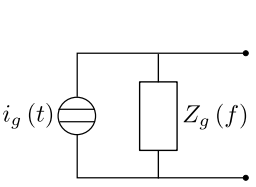
\includegraphics[width=0.8\linewidth]{gen_c.png}
                \caption*{Gen. corrente}
                \end{figure}
            \end{minipage}
            \hspace{5pt}
            \vrule
            \hspace{5pt}
            \begin{minipage}[t]{0.49\textwidth}
            \centering
                \begin{figure}[H]
                \centering
                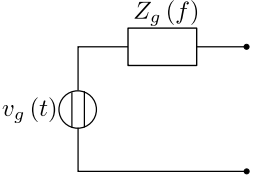
\includegraphics[width=0.85\linewidth]{gen_v.png}
                \caption*{Gen. tensione}
                \end{figure}
            \end{minipage}
        \end{figure}

        \begin{itemize}
            \item $v_g$ gen. di tensione ideale
            \item $i_g$ gen. di corrente ideale
            \item $Z_g$ impedenza interna del generatore\newline
        \end{itemize}

    \item \textbf{Bipolo passivo}

        Usato per rappresentare il carico.

        \begin{figure}[ht]
            \centering
            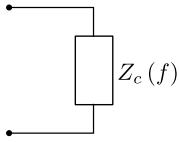
\includegraphics[width=0.3\linewidth]{pass.png}
        \end{figure}

        \begin{itemize}
            \item $Z_c$ impedenza del carico
        \end{itemize}

    \newpage

    \item \textbf{Rete 2 porte passiva}

        Usata per modellare un filtro o un mezzo trasmissivo.

        \begin{figure}[ht]
            \centering
            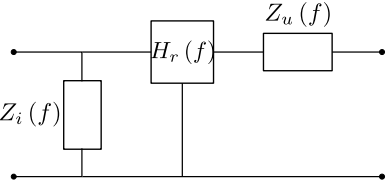
\includegraphics[width=0.6\linewidth]{2p.png}
        \end{figure}

        \begin{itemize}
            \item $Z_i$ impedenza di ingresso
            \item $H_r$ funzione di trasferimento
            \item $Z_u$ impedenza di uscita\newline
        \end{itemize}

    \item \textbf{Rete 2 porte attiva}

        Generalmente usata per modellare un amplificatore.

        \begin{figure}[ht]
            \centering
            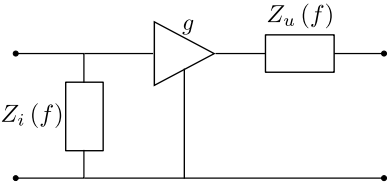
\includegraphics[width=0.6\linewidth]{2a.png}
        \end{figure}

        La differenza con il precedente sta nella trasformazione, in questo caso $H_r$ ha guadagno $g>1$.\newline
    
\end{itemize}

\noindent Nel complesso si può rappresentare un intero collegamento con:
\begin{enumerate}
    \item Bipolo attivo
    \item Cascata di $N$ reti 2 porte
    \item Bipolo passivo\newline
\end{enumerate}

\noindent Per poter calcolare la potenza su $Z_c$ o su una generica $Z_{i_k}$ si sfrutta il teorema di Thevenin, esso permette di rappresentare gli elementi a monte come un generatore equivalente con la sua impedenza e quelli a valle come un carico equivalente pari all’impedenza di ingresso del primo elemento a valle del punto di interesse.

\newpage

\noindent Dato:

\begin{figure}[ht]
    \centering
    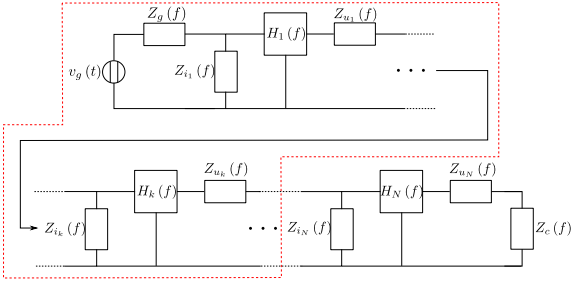
\includegraphics[width=\linewidth]{ex1.png}
\end{figure}

\noindent Ottengo:

\begin{figure}[ht]
    \centering
    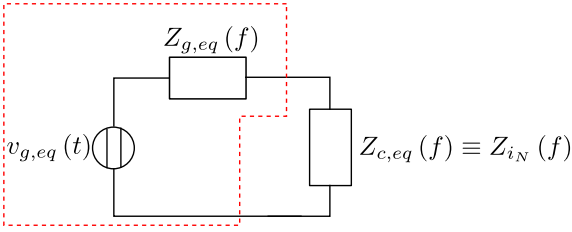
\includegraphics[width=0.8\linewidth]{ex2.png}
\end{figure}

\vspace{5pt}

\noindent A questo punto considerando $Z_c=R_c+iX_c$, $v_c$ la tensione ai suoi capi e $P_{v_c}$ lo spettro di densità di potenza del segnale ottengo la potenza assorbita dal carico con:
$$W_{Z_c}=\int_{-\infty}^{+\infty}W_{Z_c}(f)\ df=\int_{-\infty}^{+\infty}P_{v_c}\frac{R_c(f)}{|Z_c(f)|^2}\ df$$\newline

\noindent La tensione $v_c$ è ricavabile da $v_g$ tramite il partitore di tensione:
$$\frac{Z_c(f)}{Z_g(f)+Z_c(f)}$$
\noindent Essendo dipendente dalla frequenza induce però una distorsione, per evitarla deve essere:
$$Z_c(f)=Z_g(f)\frac{K}{1-K}$$
\noindent Se $K$ è tale che $Z_c(f)=Z_g(f)$ il carico è detto adattato al generatore.

\noindent Se invece $Z_c(f)=Z_g^*(f)$ si è in condizioni di MTP, $W_{Z_c}(f)$ diventa:
$$\frac{P{v_g}(f)}{4R_g(f)}\equiv W_{d_g}$$\newline

\noindent Il guadagno di una rete è dato da:
$$G=\frac{W_{Z_c}^r}{W_{Z_c}}$$
\noindent Con:
\begin{itemize}
    \item $W_{Z_c}^r$ potenza trasferita in presenza della rete
    \item $W_{Z_c}$ potenza trasferita direttamente\newline
\end{itemize}

\noindent In caso di MTP:
$$G=\frac{R_g}{R_u}|H_r|^2|H_i|^2$$\newline

\subsection{Condizioni di banda stretta}

Ci si trova in condizioni di banda stretta se dati $B$ banda del segnale e $f_p$ frequenza centrale intorno alla quale il segnale occupa $2B$ Hz si verifica:
$$2B\ll f_p$$
\noindent In questo caso si possono assumere le grandezze dipendenti dalla frequenza come costanti nell'intervallo $2B$ centrato su $f_p$.\newline

\noindent Quindi:
$$W_{Z_c}=P_{v_c}\frac{R_c}{(R_c)^2+(X_c)^2}$$
\noindent Nel caso MTP $\displaystyle W_{Z_c}=\frac{P_{v_g}}{4R_g}$.

\newpage

\section{Rumore termico}

\begin{figure}[ht]
    \centering
    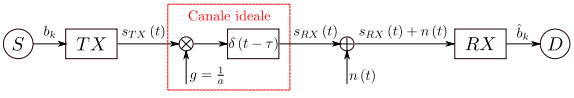
\includegraphics[width=\linewidth]{model.png}
    \caption{Modello generale di collegamento}
\end{figure}

\noindent Per valutare le prestazioni di un sistema si prende in considerazione il rapporto segnale/rumore:
$$SNR=\frac{W_R}{W_N}$$\newline

\noindent Per calcolare $W_N$ bisogna partire dal segnale del rumore $n(t)$, nella meccanica quantistica si tratta come un processo stocastico con spettro:
$$ P_N(f)=2R\frac{ h|f|}{e^{\displaystyle \frac{h|f|}{kT}-1}}\ \ [V^2/Hz]$$
\noindent Dove:
\begin{itemize}
    \item $h=6.62*10^{-34}$ J/Hz (Boltzmann)
    \item $k=1.38*10^{-23}$ J/K (Planck)
    \item $T$, temperatura in Kelvin
    \item $R$, impedenza puramente resistiva\newline
\end{itemize}

\noindent Così facendo si ottiene la tensione a vuoto su una resistenza $R$, si può quindi rappresentare la stessa come un generatore di tensione con in serie una resistenza ideale a $0K$.\newline

\noindent Si può quindi calcolare la densità di potenza:
$$W_{d_n}(f)=\frac{P_N(f)}{4R}\ \ [W/Hz]$$

\noindent Se $h|f|\ll kT$ si può approssimare $e^x\approx x+1$ per $x\ll 1$ che porta a $\frac{1}{2}kT$.\newline

\noindent Ovviamente $W_{d_n}=\int_{-\infty}^{+\infty}W_{d_n}(f)$, la presenza di un filtro in ricezione permette di "tagliare" il rumore facendo passare solo quello nell'intervallo $[-B,B]$ che porta a $kTB$.\newline

\newpage 

\noindent Dando per buono quello visto fin'ora il rumore ha le seguenti caratteristiche:
\begin{itemize}
    \item È \textbf{bianco}, i campioni presi in istanti diversi non sono correlati
    \item È \textbf{gaussiano}, il suo valore in ogni momento è la somma di molti fattori ($\sigma_0^2=N_0B=kT_0B$)\newline
\end{itemize}

\noindent Avendo una potenza estremamente piccola si considera solo se il segnale utile è molto piccolo, tipicamente all'uscita del canale:
$$y(t)=r(t)+n(t)=\frac{s(t-\tau)}{a}+n(t)$$
\noindent Con potenza:
$$P_Y=\frac{P_S}{A}+P_N$$\newline

\df Si definisce così il modello AWGN.

\subsection{Nel modello}

\begin{itemize}
    \item Bipolo passivo

    \begin{figure}[ht]
        \centering
        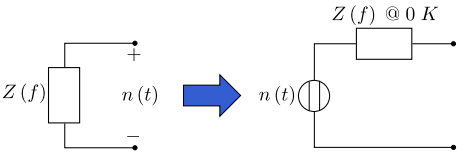
\includegraphics[width=0.7\linewidth]{r1.png}
    \end{figure}

    \[\begin{cases}
         P_N(f)=2R(f)kT\\
        \displaystyle W_{d_n}(f)=\frac{kT}{2}
    \end{cases}\]

    \item Bipolo attivo

    \begin{figure}[ht]
        \centering
        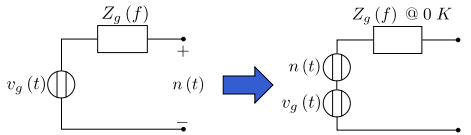
\includegraphics[width=0.7\linewidth]{r2.png}
    \end{figure}

    Con $Z_g(f)=R_g(f)+iX_g(f)$:

    \[\begin{cases}
         P_N(f)=2R_g(f)kT_g\\
        \displaystyle W_{d_n}(f)=\frac{1}{2kT_g}
    \end{cases}\]

    \item Rete 2 porte

    \[\begin{cases}
        \displaystyle P_{N,i}(f)=2R_gkT_{si}\\
        \displaystyle P_{N,u}(f)=2R_ukT_{su}\\
         W_{d_n,i}(f)=\frac{\displaystyle k(T_g+T_i)}{2}\\
         W_{d_n,u}(f)=\frac{\displaystyle k(GT_g+T_u)}{2}
    \end{cases}\]

    Con:
    \begin{itemize}
        \item $T_{si}$ temperatura di sistema all'ingresso della rete
        \item $T_{su}$ temperatura di sistema all'uscita della rete
        \item $T_g$ temperatura associata al contributo di rumore del generatore
        \item $T_u$ temperatura associata al contributo di rumore della rete
        \item $T_i$ temperatura associata al contributo di rumore della rete riportato in ingresso alla stessa\newline
    \end{itemize}

    Il rumore introdotto da una rete si può quantificare tramite il fattore di rumore:
    $$F=1+\frac{T_i}{T_0}$$
    \noindent Se la rete è passiva coincide con l'attenuazione.\newline

    In caso di più reti in cascata si calcola il fattore totale come:
    $$F_{TOT}=F_1+\frac{(F_2-1)}{G_1}+\frac{(F_3-1)}{G_1G_2}+\ldots$$\newline
    
    La temperatura in ingresso al ricevitore sarà quindi:
    $$\text{temp. mezzo}+(F_{TOT-1})T_0$$\newline

    Integrando su $[-B,B]$ nel caso $T_m=T_0$ si ottiene:
    $$W_N=kF_{TOT}T_0B$$
    
\end{itemize}

\section{Modulazioni}

\df La modulazioine è un'operazione di adattamento del segnale al canale.\newline

\subsection{Portante impulsiva}

La modulazione su portante impulsiva associa i simboli generati dalla sorgente ad un segnale tempo-continuo formato da una sequenza di impulsi spaziati dal tempo di simbolo $T_L$:
$$s(t)=\sum_kv_kg(t-kT_L)$$
\noindent Con:
\begin{itemize}
    \item $v_k$ valore di tensione associato al simbolo generico
    \item $g(t)$ impulso usato\newline
\end{itemize}

\noindent(Da qui in poi si assuma una modulazione a 2 livelli e bit singoli come simboli)\newline

\noindent Il procedimento di associazione si può dividere in 2 fasi:

\begin{figure}[ht]
    \centering
    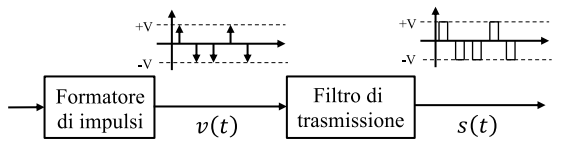
\includegraphics[width=0.8\linewidth]{mod_imp.png}
\end{figure}

\noindent In cui:
\begin{itemize}
    \item Il formatore di impulsi associa alla sequenza di bit un segnale analogico formato da una sequenza di impulsi di Dirac di ampiezza $\pm V$ e spaziati di $T_b=T_L$:

        $$v(t)=\sum_kv_k\delta(t-kT_L)$$

    \item Il filtro effettua la convoluzione di $v(t)$ con la sua risposta impulsiva $g(t)$:

    $$s(t)=v(t)*g(t)=\sum_kv_kg(t-kT_L)$$\newline
    
\end{itemize}

\noindent Resta da scegliere $g(t)$, il metodo più intuitivo è scegliere un impulso di durata $\leq T_L$:
\begin{enumerate}
    \item $NZR$, l'impulso occupa tutto il periodo di bit
    \item $ZR$, l'impulso ha durata minore e torna a 0 tra gli impulsi\newline
\end{enumerate}

\noindent Il problema di entrambi sta nel fatto che avendo impulsi di durata limitata presentano banda infinita, per ovviare al problema si sceglie un impulso con le caratteristiche opposte ma in questo caso si può verificare interferenza tra i simboli.\newline

\noindent Per non introdurre interferenza intersimbolica $g(t)$ deve rispettare le condizioni di Nyquist:
\begin{itemize}
    \item Nel tempo

        \[g(jT_L)=\begin{cases}
            1 & j=0\\
            0 & j\neq 0
        \end{cases}\]

    \item Nella frequenza

        $$\sum_kG(f-\frac{k}{T_L})=T_L$$\newline
    
\end{itemize}

\noindent Una famiglia di funzioni che rispetta queste condizioni sono quelle a coseno rialzato:
\[G(f)=\begin{cases}
    T_L & 0\leq|f|\leq\frac{F_L}{2}(1-\gamma)\\
    \frac{T_L}{2}(1+\cos({\frac{\pi T_L}{\gamma}(|f|-\frac{f_L}{2}(1-\gamma)))}) & \frac{f_L}{2}(1-\gamma)<|f|\leq\frac{f_L}{2}(1+\gamma)\\
    0 & |f|>\frac{f_L}{2}(1+\gamma)
\end{cases}\]

\noindent Con risposta impulsiva:

$$ g(t)=g_{min}(t)\left[\frac{\displaystyle\cos(\frac{\pi\gamma t}{T_L})}{1-(\frac{\displaystyle\gamma2t}{T_L})^2}\right]$$

\begin{figure}[ht]
    \centering
    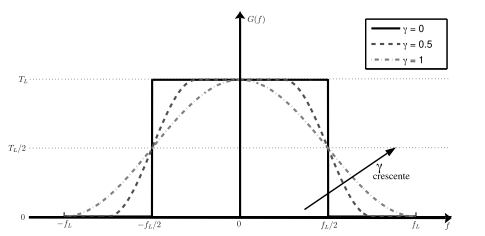
\includegraphics[width=0.8\linewidth]{cos.png}
\end{figure}

\newpage

\noindent Si nota facilmente che al variare di $\gamma$ l'area resta identica, quindi la banda occupata risulta $\frac{f_L}{2}(1+\gamma)$.\newline

\noindent Avendo una correlazione tra banda e tempo di simbolo si può adesso generalizzare per più di 2 livelli:

\begin{table}[ht]
    \centering
    \begin{tabular}{c|c}
        Bit & Simbolo\\
         \hline
        00 & $V_1$\\
        01 & $V_2$\\
        10 & $V_3$\\
        11 & $V_4$\\
    \end{tabular}
\end{table}

\noindent $T_L=2T_b,\ f_L=\frac{f_b}{2}$, la banda sarà la metà rispetto a quella a 2 livelli.\newline

\noindent A livello generale si possono associare sequenze di $k$ bit a sequenze di $N$ simboli su alfabeto di $L$ elementi, quindi $2^k\rightarrow L^N$, dovendo esserci una corrispondenza univoca deve essere $2^k\leq L^N$. Nel caso sia strettamente minore si introduce un parametro di ridondanza che fornisce "l'abbondanza" di sequenze di simboli rispetto alle sequenze di bit da codificare:
$$\rho=\frac{N\log_2(L-k)}{N\log_2L}$$\newline

\noindent Si può introdurre questo valore nella relazione tra banda e bit-rate:
$$\frac{f_L}{f_b}=\frac{N}{k}=\frac{1}{(1-\rho)\log_2L}\rightarrow B=\frac{f_b(1+\gamma)}{2(1-\rho)\log_2L}$$

\newpage

\subsubsection{Probabilità d'errore}

\begin{figure}[ht]
    \centering
    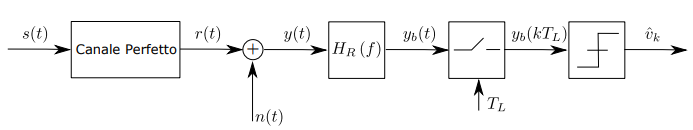
\includegraphics[width=\linewidth]{err.png}
    \caption{Schema considerato}
\end{figure}

\noindent Transito del segnale:
\begin{enumerate}
    \item $s(t)\rightarrow r(t)$

        Il canale introduce:
            \begin{itemize}
                \item Attenuazione
                \item Ritardo di propagazione
                \item Distorsione
            \end{itemize}

    \item $r(t)\rightarrow y(t)$

    $y$ dato da $r(t)+n(t)$.

    \item $y(t)\rightarrow y_b(t)$

        Il filtro lascia passare il segnale utile e riduce l'effetto dei disturbi.

    \item $y_b(t)\rightarrow y_b(kT_L)$

        Il campionatore fornisce un campione ogni $kT_L$ secondi.

    \item $y(kT_L)\rightarrow \hat{v_k}$

        Il decisore a soglia scegliera la soglia più adatta tra quelle presenti.\newline
    
\end{enumerate}

\noindent Nel caso $L=2$ sarà presente una sola soglia $V_d$ e due possibili valori $V_0,V_1$ associati a $b_k=0,b_k=1$. La probabilità d'errore si può scrivere come:
$$P_e=P\{y_b(kT_L)\leq V_d|\ b_k=1\}P\{b_k=1\}+P\{y_b(kT_L)>V_d|\ b_k=0\}P\{b_k=0\}$$\newline

\noindent $y_b(kT_L)$ è dato dalla somma $r_b(kT_L)+n_b(kT_L)$ dove:

\[r_b(kT_L)=\begin{cases}
    r_1 & b_k=1\\
    r_0 & b_k=0
\end{cases}\]

\[n_b(kT_L)\text{ è una v.a. gaussiana }\begin{cases}
    E[n_b]=0\\
    \sigma_{n_b}^2=\sigma_0^2
\end{cases}\]

\noindent Fissato $b_k$ $r_b$ diventa una costante e $y_b$ diventa una v.a gaussiana:

\[\begin{cases}
    E[y_b]=r_b\\
    \sigma_{y_b}^2=\sigma_0^2
\end{cases}\]\newline

\df La funzione di errore complementare ($erfc(y)$) è definita come:
$$\frac{2}{\pi}\int_y^{+\infty}e^{-\varepsilon^2}\ d\varepsilon$$\newline

\noindent Assumendo che ci sia equiprobabilità la formula risulta:
$$P_e=\frac{1}{2}\left[\frac{1}{2}erfc(-\frac{V_d-r_1}{\sqrt{2}\sigma_0})\right]+\frac{1}{2}\left[\frac{1}{2}erfc(-\frac{V_d-r_0}{\sqrt{2}\sigma_0})\right]$$\newline

\noindent $\displaystyle\frac{r_1+r_0}{2}$ fornisce la soglia ideale, in questo caso la probabilità d'errore diventa:
$$P_e=\frac{1}{2}erfc(\frac{r_1-r_0}{2\sqrt{2\sigma_0}})$$
\noindent Generalmente $y^2=\frac{SNR}{2}$.\newline

\noindent Nel caso multilivello si hanno $L-1$ soglie distinte in interne ed esterne, il posizionamento migliore è quello con soglie equidistanti tra livelli adiacenti.\newline

\noindent Vale:
\begin{itemize}
    \item $\displaystyle V_{d_i}=\frac{r_{i+1}+r_i}{2}$ per $i\in[0,L-2]$
    \item $\displaystyle\Delta=\frac{r_{L-1}-r_0}{L-1}$
    \item $\displaystyle V_{d_i}-r_i=r_{i+1}-V_{d_i}=\frac{\Delta}{2}$ per $i\in[0,L-2]$
    \item $\displaystyle P_e=(1-\frac{1}{L})erfc\left(\frac{r_{L-1}-r_0}{(L-1)2\sigma_0\sqrt{2}}\right)$
    \item $\displaystyle y^2=\frac{3SNR}{2(L^2-1)}$
\end{itemize}

\newpage

\subsection{Portante sinusodiale}

Queste modulazioni si usano per segnali analogici tipicamente in banda base le cui caratteristiche spettrali sono note o caratterizzabili, tipicamente si considerano segnali limitati in banda reali o complessi.\newline

\noindent Lo scopo principale è trasportare lo spettro del segnale modulante $m(t)$ intorno ad una frequenza adatta al mezzo trasmissivo usato, ciò avviene associando ad $m(t)$ uno dei parametri del segnale portante oscillante a $f_p$:
\begin{itemize}
    \item \textbf{Ampiezza}
    \item \textbf{Frequenza}
    \item \textbf{Fase}\newline
\end{itemize}

\noindent Il generico segnale $m(t)=m_1(t)+im_2(t)$ verrà trasformato con il seguente procedimento:
\begin{enumerate}
    \item \textbf{Modulazione}, $f_1\{m_1(t)\}+if_2\{m_2(t)\}$
    \item \textbf{Traslazione}, $s^+(t)=(f_1\{m_1(t)\}+if_2\{m_2(t)\})e^{i(2\pi f_pt+\varphi_0)}$

        Se l'intervallo di banda occupato è minore della frequenza portante il segnale avra solo contributi a frequenze positive.\newline
\end{enumerate}

\noindent Il segnale modulato è dato dalla parte reale di $s^+(t)$ (dopo i calcoli):
$$f_1\{m_1(t)\}\cos(2\pi f_pt+\varphi_0)-f_2\{m_2(t)\}\sin(2\pi f_pt+\varphi_0)$$

\noindent Se $m(t)$ è reale non è presente la seconda parte.\newline

\noindent La portante si può scegliere in 2 modi:
\[\begin{cases}
    A\cos(2\pi f_pt+\varphi_0) & \text{In fase}\\
    A\sin(2\pi f_pt+\varphi_0) & \text{In quadratura}
\end{cases}\]

\noindent Avendo solo lo spettro di fase diverso la potenza è per entrambe $\frac{A^2}{2}\ V^2$.\newline

\df Il segnale $\ubar{s}(t)=f_1\{m_1(t)\}+if_2\{m_2(t)\}=s_f(t)+is_q(t)$ è detto inviluppo complesso, $s_f,s_q$ sono dette componenti analogiche di bassa frequenza rispettivamente in
fase e in quadratura.\newline

\subsubsection{AM}

Nella modulazione AM l'ampiezza della portante sarà proporzionale al segnale $m(t)$, usando la portante in fase si ottiene:
$$s(t)=k_am(t)\cos(2\pi f_pt+\varphi_0)$$
\noindent Risulta però comodo in ricezione avere l'inviluppo sempre positivo, quindi si somma a $k_a$ un valore $a_p$, in base al valore di quest'ultimo si distinguono:
\begin{itemize}
    \item Portante soppressa ($a_p=0$)
    \item Portante ridotta ($0<a_p\leq max\{k_a|m(t)|\}$)
    \item Portante intera ($a_p>max\{k_a|m(t)|\}$)
\end{itemize}

\noindent In ogni caso l'inviluppo è $\ubar{s}(t)=a_p+k_am(t)$.\newline

\noindent Lo spettro del segnale modulato dipende da $m(t)$, 3 possibili casi:
\begin{enumerate}
    \item Sinusoide
        \begin{itemize}
            \item $m(t)=A\cos(2\pi Wt)$
            \item $s(t)=k_aA\cos(2\pi Wt)\cos(2\pi f_pt+\varphi_0)+a_p\cos(2\pi f_pt+\varphi_0)$
            \item $P_M=\frac{A^2}{2}$
        \end{itemize}

        $$P_{AM-PI}=\frac{k_a^2\frac{A^2}{2}}{2}+\frac{a_p^2}{2} \text{ con }\frac{k_a^2\frac{A^2}{2}}{2}<\frac{a_p^2}{2}$$
        $$P_{AM-PR}\ \text{ come il precedente ma } 0<\frac{a_p^2}{2}\leq\frac{k_a^2\frac{A^2}{2}}{2}$$
        $$P_{AM-PS}\ \text{ come $PI$ ma con solo la prima parte}$$

    Con portante intera e ridotta una parte della potenza viene "sprecata", la frazione di potenza utile è pari a:
    $$\eta=\frac{\displaystyle\frac{k_a^2P_M}{2}}{\displaystyle\frac{k_a^2P_M}{2}+\frac{a_p^2}{2}}$$

    \[\begin{cases}
        \eta<0.5 & \text{Intera}\\
        0.5\leq\eta<1 & \text{Ridotta}\\
        \eta=1 & \text{Soppressa}
    \end{cases}\]

    \newpage
    
    \item Segnale deterministico di banda $B$
    
        Ipotizzando:
        \begin{itemize}
            \item $m(t)$ reale
            \item $m(t)$ a valor medio nullo
        \end{itemize}

        $$P_{AM-PI-PR}(f)=\frac{k_a^2}{4}(e^{i\varphi_0}M(f-f_p)+e^{-i\varphi_0}M(f+f_p))+\frac{a_p}{2}(e^{i\varphi_0}M(f-f_p)+e^{-i\varphi_0}M(f+f_p))$$

        $$P_{AM-PS}(f)\ \text{ come il precedente ma con solo la prima parte}$$
    
    \item Realizzazione di un processo di banda $B$
        \begin{itemize}
            \item Processo WSS
            \item Media nulla
        \end{itemize}

        $$P_S(f)=\frac{k_a^2}{4}(P_M(f-f_p)+P_M(f+f_p))+\frac{a_p^2}{4}(\delta(f-f_p)+\delta(f+f_p))$$\newline
    
\end{enumerate}

\noindent Dall'ultima formula risulta che è presente una replica a $-f_p$, un segnale di questo tipo è detto a banda laterale doppia.\newline

\noindent Il filtro di Hilbert causa uno sfasamento di $\frac{\pi}{2}$ al segnale, sommando/sottraendo il risultato al segnale originale si elimina una delle bande:
$$s(t)=k_am(t)\cos(2\pi f_pt)\pm k_am_h(t)\sin(2\pi f_pt)$$\newline

\noindent Il filtro di Hilbert non è fisicamente realizzabile, esistono però dei filtri che lo approssimano riducendo molto una delle bande, così facendo si ottiene un segnale a banda ridotta.

\newpage

\noindent Esistono 3 tipi di demodulatori:
\begin{itemize}
    \item \textbf{Inviluppo} (solo PI)

    \begin{figure}[ht]
        \centering
        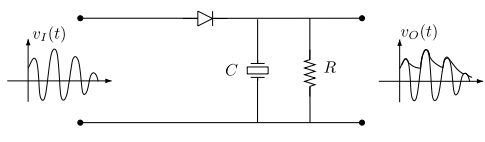
\includegraphics[width=0.7\linewidth]{inv.png}
    \end{figure}
    
    \item \textbf{Omodina} (meglio PR)

    \begin{figure}[ht]
        \centering
        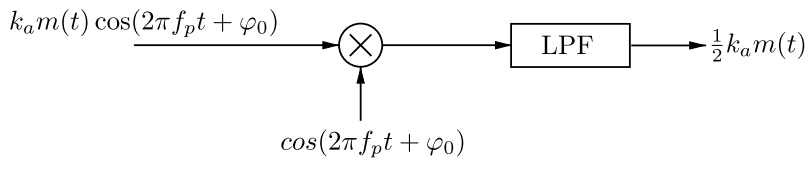
\includegraphics[width=0.8\linewidth]{omo.png}
    \end{figure}

    \begin{itemize}
        \item Richiede una stima di frequenza e fase della portante
        \item Il segnale uscente dal mixer è:

        $$k_am(t)\left[\frac{1+\cos(2(2\pi f_pt+\varphi_0))}{2}\right]$$

        \item Il filtro passa basso con $f_c\ll 2f_p$ toglierà la componente sinusoidale
        
    \end{itemize}
    
    \item \textbf{Eterodina}

    \begin{figure}[ht]
        \centering
        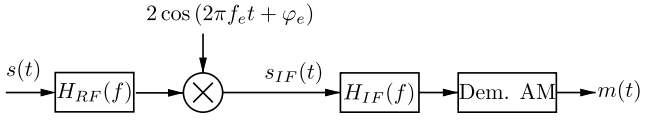
\includegraphics[width=0.8\linewidth]{ete.png}
    \end{figure}

    \begin{itemize}
        \item $H_{RF}$ deve attenuare fortemente la frequenza $f_p-2f_e$
        \item $f_e$ è scelta in modo che $f_p+f_e$ e $f_p-f_e$ siano distanti
        \item Il filtro $H_{IF}$ rimuove $f_p+f_e$
        \item $m(t)$ è uguale ma centrato su $f_p- f_e$
        \item Si può ora demodulare con uno degli altri demodulatori
    \end{itemize}
    
\end{itemize}

\newpage

\subsubsection{Angolari}

Nelle modulazioni angolari il modulante determina la fase istantanea della portante, si ha:
$$s(t)=a\cos(2\pi f_pt+\varphi_0+\alpha(t))$$
\noindent Con potenza $\frac{a^2}{2}$.\newline

\noindent Per associare $\alpha(t)$ a $m(t)$ ci sono 2 modi:
\begin{enumerate}
    \item Mod. di fase (PM)

        $$\alpha(t)=k_\phi m(t)$$
    
    \item Mod. di frequenza (FM)

        $$\alpha(t)=2\pi k_F\int m(\tau)\ d\tau$$\newline
    
\end{enumerate}

\noindent Per capire le proprietà spettrali si riscrive $s(t)$:
$$\frac{a}{2}\left[e^{i(2\pi f_pt+\varphi_0)}e^{i\alpha(t)}+e^{-i(2\pi f_pt+\varphi_0)}e^{-i\alpha(t)}\right]$$

\noindent Nel caso $\text{(banda di }e^{i\alpha(t)})\ll f_p$:
$$s^+(t)=\frac{a}{2}e^{i\alpha(t)}[e^{i(2\pi f_pt+\varphi_0)}]\text{ (uguale per l'altro termine)}$$\newline

\noindent Si può quindi rappresentare $e^{i\alpha(t)}$ come la serie:
$$\sum_{k=0}^{+\infty}\frac{1}{k!}(i\alpha(t))^k$$
\noindent Che tipicamente si arresta dopo un certo numero di termini.\newline

$$\text{maggiore è }\alpha(t)\rightarrow\text{ più grande è la banda di }e^{i\alpha(t)}$$

\newpage

\noindent Come per l'AM:
\begin{itemize}
    \item \textbf{Sinusoide}

        $$m(t)=A\cos(2\pi Wt)$$

        \[\begin{cases}
            \alpha(t)=K_\phi A\cos(2\pi Wt) & PM\\
            \alpha(t)=\frac{k_F}{W}A\sin(2\pi Wt) & FM
        \end{cases}\]

        \[\text{Indici di modulazione}\begin{cases}
            I_P=K_\varphi A & PM\\
            I_F=\frac{k_F}{W}A & FM
        \end{cases}\]

        In generale $\ubar{s}(t)=ae^{i\alpha(t)}$, nel caso FM:
        $$\ubar{s}(t)=a\sum_{k=-\infty}^{+\infty}J_K(\frac{k_F}{W}A)e^{i2\pi kWt}$$
        Con $J_K()$ funzione di Bessel del primo tipo di ordine $k$.\newline

        Lo spettro sarà:
        $$a\sum_{k=-\infty}^{+\infty}J_K(\frac{k_F}{W}A)\delta(f-kW)$$\newline

        La densità di energia invece:
        $$a^2\sum_{k=-\infty}^{+\infty}|J_K(\frac{k_F}{W}A)|^2\delta(f-kW)$$\newline

        La banda dell'inviluppo si approssima con la banda di Carson:
        $$B_C\approx W(I_F+1)$$
        Guardando lo spettro di densità di potenza sul piano si vede che c'è un'occupazione di banda di larghezza $2B_C$ intorno a $f_p$ e $-f_p$, quindi la banda totale occupata è $4B_C$.

    \newpage
        
    \item \textbf{Segnale generico}
    
        \begin{itemize}
            \item $m(t)$
            \item Banda $B$
            \item Media nulla\newline
        \end{itemize}
    
        2 casi:
            \begin{enumerate}
                \item Basso indice di modulazione

                    \[\text{Spettro }\begin{cases}
                        k_\varphi M(f) & PM\\
                        \frac{\displaystyle2\pi k_F}{\displaystyle i2\pi f}M(f) & FM
                    \end{cases}\]
                
                \item Alto indice di modulazione

                    $$\uparrow k_F\rightarrow\uparrow B_{TOT}$$\newline
                
            \end{enumerate}
\end{itemize}

\noindent La demodulazione di un segnale FM si svolge nel seguente modo:\newline

\noindent Dato $s(t)$ modulato d'angolo, si ha:
$$\frac{ds(t)}{dt}=-a[2\pi f_p+\frac{d\alpha(t)}{dt}]\sin(2\pi f_pt+\alpha(t))$$
\noindent Nel caso FM diventa:
$$\sin(2\pi f_pt+\alpha(t))(-a2\pi f_p-a2\pi k_Fm(t))$$
\noindent Ponendo:
\begin{itemize}
    \item $a_p=-a2\pi f_p$
    \item $k_a=-a2\pi k_F$
\end{itemize}
\noindent Ed essendo $k_F\ max\{|m(t)|\}\ll f_p$ risulta $a_p>k_a$, quindi è un segnale AM-PI.\newline

\begin{figure}[ht]
    \centering
    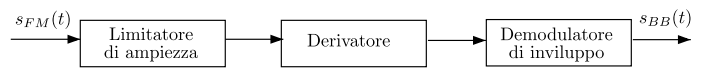
\includegraphics[width=\linewidth]{dem.png}
    \caption{Schema demodulatore FM}
\end{figure}

\noindent $S_{BB}(t)=a2\pi f_p+a2\pi k_Fm(t)$ da cui si può estrarre $m(t)$.

\subsubsection{Confronto delle prestazioni}
\begin{itemize}
    \item $SNR_{dem}$ è l'SNR a valle del demodulatore
    \item $SNR_{mod}$ è l'SNR prima della demodulazione
    \item $SNR_{rif}$ è l'SNR che si avrebbe senza modulazione\newline
\end{itemize}

\noindent Casi:
\begin{itemize}
    \item \textbf{AM-BLD-PI/PR}

        $$SNR_{dem}=\eta SNR_{rif}$$
        $$SNR_{mod}=\frac{\eta SNR_{rif}}{2}$$

    \item \textbf{AM-BLD-PS}

        $$SNR_{dem}=SNR_{rif}$$
        $$SNR_{mod}=\frac{SNR_{rif}}{2}$$

    \item \textbf{AM-BLU}

        $$SNR_{dem}=SNR_{rif}=SNR_{mod}$$

    \item \textbf{FM/PM}

        $$SNR_{dem}=3I_F^2SNR_{rif}$$\newline

\end{itemize}

\noindent\textbf{Le valutazioni sono fatte a parità di potenza ricevuta, usando la stessa formula per il rumore ed usando un filtro $H_{RX}(f)$ che lascia passare solo la banda usata dal segnale di interesse.}\newline

\newpage

\subsection{Numeriche}

Un approccio più generale consiste nel generare un segnale che costituisce l'inviluppo complesso del segnale modulato $s(t)=s_f(t)+is_q(t)$ (BLD-PS), esso definirà una traiettoria nel piano complesso su cui si definiscono i simboli.\newline

\noindent Il valore dell'inviluppo deve essere imposto solo in $t=kT_L$ con $k\in(-\infty,+\infty)$ e $T_L$ periodo di simbolo, negli altri istanti può assumere qualsiasi valore.\newline

\begin{figure}[ht]
    \centering
    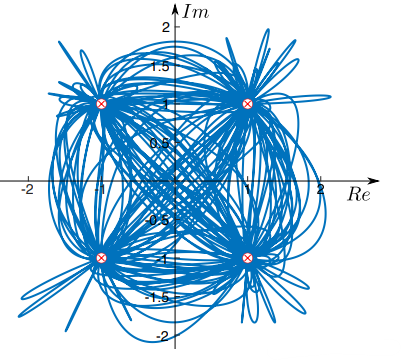
\includegraphics[width=0.5\linewidth]{num.png}
    \caption{Esempio di andamento}
    \label{fig:qam4}
\end{figure}

\df L'insieme $L$ dei punti sul piano complesso assunti da $\ubar{s}(t)$ in $kT_L$ è detto costellazione della modulazione.\newline

\noindent Alcune modulazioni:
\begin{itemize}
    \item \textbf{BPSK}, equivalente della modulazione antipodale, $L=2$

        \[\ubar{s}(kT_L)\equiv\ubar{s}(kT_b)=\begin{cases}
            A & b_k=1\\
            -A & b_k=0
        \end{cases}\]

        \begin{figure}[ht]
            \centering
            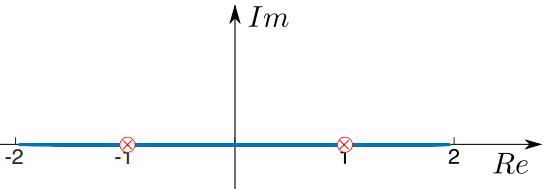
\includegraphics[width=0.7\linewidth]{bpsk.png}
            \caption{Andamento con $A=1\ V$}
        \end{figure}

    Risulta $P_s=\frac{A^2}{2}$.

    \item \textbf{OOK}

        Come la precedente ma $b_k=0\Rightarrow0$, $P_S=\frac{A^2}{4}$.

    \item \textbf{QAM}, estensione della multilivello

        La costellazione è una griglia regolare di lato $\sqrt{L}$, la Figura \ref{fig:qam4} è una QAM-4.

    \begin{figure}[ht]
        \centering
        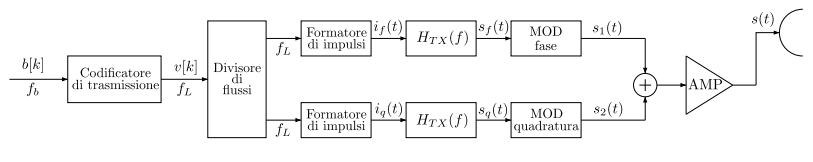
\includegraphics[width=\linewidth]{qam.png}
        \caption{Schema di trasmissione QAM}
    \end{figure}

    \begin{itemize}
        \item $f_L=\displaystyle\frac{f_b}{\log_2L}$ su ogni ramo
        \item $B=(1+\gamma)\displaystyle\frac{f_b}{2\log_2L}$
    \end{itemize}

    \item \textbf{PSK}

        Ogni simbolo viene associato ad un valore di fase dato da:
        $$\varphi_I=(2I+1)\frac{\pi}{L}\text{ con } I\in[0,L-1]$$

        Quindi $\ubar{s}(kT_L)=A\cos(\varphi_k)+i\sin(\varphi_k)$

    \begin{figure}[ht]
        \centering
        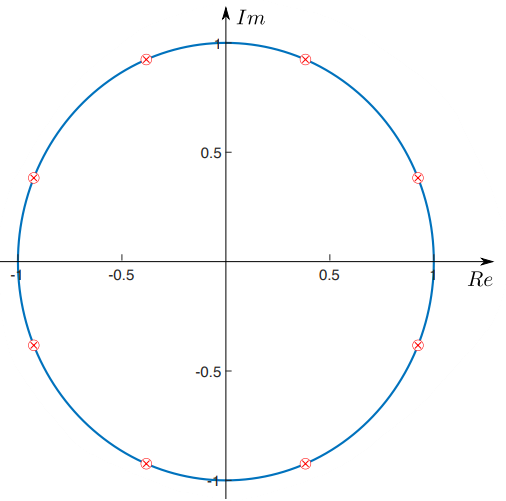
\includegraphics[width=0.5\linewidth]{psk.png}
        \caption{$A=1,\ L=8$}
    \end{figure}

    \newpage

    Ci sono 3 varianti:
    \begin{enumerate}
        \item \textbf{PSK}, impulsi rettangolari per l'andamento della fase
        \item \textbf{MSK}, archi di sinusoidi per l'andamento della fase
        \item \textbf{CPM}, variazione di fase continua e inviluppo costante\newline
    \end{enumerate}
    
\end{itemize}

\noindent Le probabilità di errore sono:
\begin{itemize}
    \item \textbf{BSPK}

        $$\frac{1}{2}erfc\left(\sqrt{\frac{SNR_{rif}}{2}}\right)$$

    \item \textbf{OOK}

        $$\frac{1}{2}erfc\left(\sqrt{\frac{SNR_{rif}}{4}}\right)$$

    \item \textbf{QAM}

        $$\approx erfc\left(\sqrt{\frac{3}{4}\frac{SNR_{rif}}{(L-1)}}\right)$$

    \item \textbf{PSK}

        $$\approx erfc\left(\sqrt{\frac{1}{2}SNR_{rif}\sin^2\left(\frac{\pi}{L}\right)}\right)$$\newline
    
\end{itemize}

\newpage

\section{Mezzi trasmissivi}

\subsection{Radio}

Le comunicazioni radio utilizzano onde elettromagnetiche che si propagano:
\begin{itemize}
    \item Nell'atmosfera (terrestri)
    \item Nel vuoto (spaziali)
    \item In entrambi (satellitari)
\end{itemize}

\begin{figure}[ht]
    \centering
    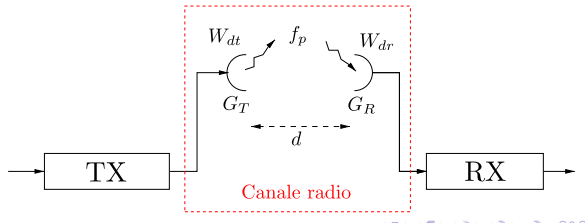
\includegraphics[width=0.7\linewidth]{radio.png}
    \caption{Schema generale}
\end{figure}

\noindent Il canale è composto da:
\begin{itemize}
    \item Antenna trasmittente
    \item Mezzo
    \item Antenna ricevente\newline
\end{itemize}

\noindent Le antennte fungono da trasduttori, ognuna ha un suo guadagno:
$$F(\theta,\phi)=\frac{W_{dt}(\theta,\phi)}{W_{dt}^i(\theta,\phi)}$$
\noindent Dove:
\begin{itemize}
    \item $W_{dt}(\theta,\phi)$ è la potenza irradiata dall'antenna nella direzione $(\theta,\phi)$
    \item $W_{dt}^i(\theta,\phi)$ è la potenza irradiata da un'antenna isotropa\newline
\end{itemize}

\noindent Si identificano 3 modi principali per propagare le onde:
\begin{enumerate}
    \item \textbf{Riflessione e diffusione}
        \begin{itemize}
            \item Riflessione $\rightarrow$ rimbalzo sulla ionosfera
                \begin{itemize}
                    \item Sotto i $30\ MHz$
                    \item Fino a 4000 Km
                \end{itemize}
            \item Diffusione
                \begin{itemize}
                    \item Frequenze tra 30 e 300 $MHz$
                    \item Distanze minori del precedente
                \end{itemize}
        \end{itemize}
    \item \textbf{Onda superficiale}

        Si usa la superficie terrestre come se fosse una guida d'onda:
            \begin{itemize}
                \item Sotto i 3 $MHz$
                \item Fino a 10000 Km
                \item Usata in particolare sull'acqua
            \end{itemize}
    
    \item \textbf{Diretta}

        Serve visibilità diretta tra le antenne, la distanza massima in Km è:
        $$3.6(\sqrt{h_{1,m}}+\sqrt{h_{2,m}})$$

        \begin{figure}[ht]
            \centering
            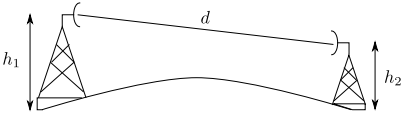
\includegraphics[width=0.7\linewidth]{dir.png}
        \end{figure}

        \begin{table}[ht]
            \centering
            \begin{tabular}{c|c}
                Standard & Max. potenza\\
                 \hline
                WiFi & 36 dBm (US), 20 dBm (EU)\\
                 \hline
                UWB & 0.55 W\\
                 \hline
                GSM & 39 dBm\\
                 \hline
                UMTS & 33 dBm \\
            \end{tabular}
            \caption{Regolazioni}
        \end{table}

        Assumendo che il canale sia ideale si può caratterizzare l'attenuazione dello spazio libero come:

        $$A_{d,dB}=10\log_{10}\left(\frac{1600\pi}{9}\right)+20log_{10}(f_{p,MHz})+20\log_{10}(d_{Km})-G_{TX,dB}-G_{RX,dB}$$

        Nella realtà però non è cosi, tipicamente il canale è selettivo in frequenza a causa dei fenomeni atmosferici ed esiste la possibilità che ci siano cammini multipli tra le antenne, ciò porta a problemi durante la ricezione.
    
\end{enumerate}

\newpage

\subsection{Cavo di rame}

\subsubsection{Doppino telefonico}

\begin{figure}[ht]
    \centering
    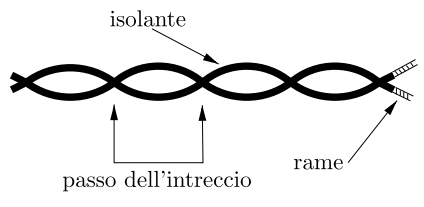
\includegraphics[width=0.5\linewidth]{dopp.png}
\end{figure}


\begin{table}[ht]
    \centering
    \begin{tabular}{|c|c|c|c|c|}
        \hline
        \multicolumn{5}{|c|}{\textbf{Analogici/misti}}\\
        \hline
        Sigla & Occ. banda positiva (KHz) & Bit rate (Kb/s) & Anno & Modulazioni\\
        \hline
        V.34 & 3.429 & 33.6 & 1994 & QAM\\
        \hline
        V.90 & 4 & 56/33.6 & 1998 & PCM+QAM\\
        \hline
        V.92 & 4 & 56/48 & 2001 & PCM\\
         \hline
        \multicolumn{5}{|c|}{\textbf{Numerici}}\\
        \hline
        - & - (MHz) & - (Mb/s) & - & -\\
        \hline
        G.961 & 0.12 & 0.144 & 1993 & ISDN\\
        \hline
        G.992 & 0.9 & 8 & 1999 & ADSL (OFDM)\\
        \hline
        G.993.1 & 8 & 55 & 2004 & VDSL1 (ODFM)\\
        \hline
        G.993.2 & 12 & 68 & 2006 & VDSL2\\
        \hline
        G.993.3 & 35 & 300 & 2015 & VDSL2 35b\\
        \hline
    \end{tabular}
    \caption{Standard}
\end{table}

\noindent Alcuni nel dettaglio:
\begin{itemize}
    \item \textbf{V.34}

        Definito considerando uno schema in cui agli estremi è presente una tratta analogica:

        \begin{figure}[ht]
            \centering
            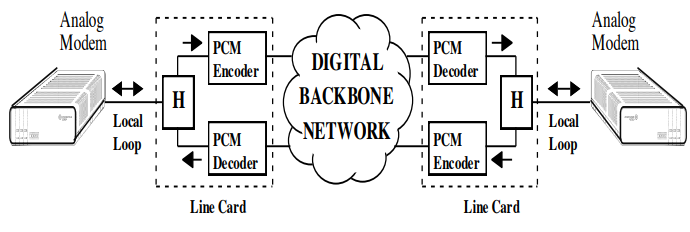
\includegraphics[width=\linewidth]{v34.png}
        \end{figure}

    \newpage

    \item \textbf{V.90}

        Introdotto per sfruttare la connessione numerica tra operatore telefonico e ISP, nella tratta analogica usa la modulazione PAM i cui livelli sono dati dal codificatore PCM. Presenta una quantizzazione non lineare per tenere in conto la dinamica della voce umana, questo limita il rate ottenibile.
        
        \begin{figure}[ht]
            \centering
            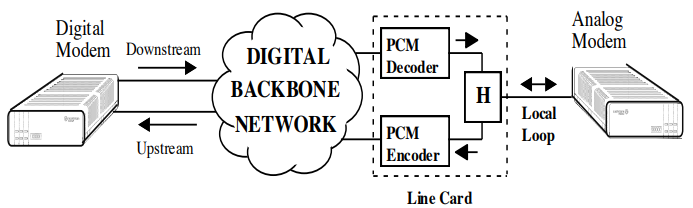
\includegraphics[width=\linewidth]{v90.png}
        \end{figure}
    
\end{itemize}

\subsubsection{Cavo coassiale}

\noindent Attualmente viene usato per:
\begin{itemize}
    \item \textbf{DVB-T2}

        Portante tra 400 e 700 $MHz$, occupazione di banda positiva $8\ MHz$
    
    \item \textbf{DVB-S2}

        Portante tra 950 e 2150 $MHz$, occupazione di banda positiva $33\ MHz$\newline
    
\end{itemize}

\begin{figure}[ht]
    \centering
    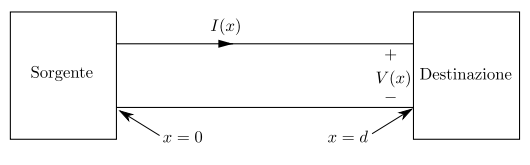
\includegraphics[width=\linewidth]{cavo.png}
    \caption{Modello generale}
\end{figure}

\noindent Indicando $V_d$ come onda diretta e $V_r$ come inversa si ha:
$$V(x)=V_de^{-\gamma(f)x}+V_re^{\gamma(f)x}$$
$$V(x)=\frac{V_de^{-\gamma(f)x}+V_re^{\gamma(f)x}}{Z_0(f)}$$

\newpage

\noindent Con le costanti secondarie:
\begin{itemize}
    \item $Z_0(f)$ impedenza caratteristica
    \item $\gamma(f)$ costante di propagazione

        Si ha $\gamma(f)=\alpha(f)+i\beta(f)$ in cui:
            \begin{itemize}
                \item $\alpha(f)$ determina l'attenuazione ($Neper/m$)
                \item $\beta(f)$ determina il ritardo ($rad/m$)\newline
            \end{itemize}
    
\end{itemize}

\noindent Le costanti primarie sono:
\begin{itemize}
    \item $R$, resistenza per unità di lunghezza ($\Omega/m$)
    \item $H$, induttanza per unità di lunghezza ($Henry/m$)
    \item $G$, conduttanza per unità di lunghezza ($Siemens/m$)
    \item $C$, capacità per unità di lunghezza ($Farad/m$)\newline
\end{itemize}

\noindent Si possono esprimere le costanti secondarie basandosi su quelle primarie:
$$Z_0(f)=\sqrt{\frac{R+i2\pi fH}{G+i2\pi fC}}$$
$$\gamma(f)=\sqrt{(RG-(2\pi f)^2CH)+(i2\pi f(RC+GH))}$$
\noindent Per $f\gg 0$ l'attenuazione ed il ritardo risultano indipendenti da $f$, la linea si comporta quindi da canale ideale.\newline

\noindent La condizione di Heaviside si verifica quando $GH=RC$, si ha:
$$\gamma(f)=\sqrt{CH}(\frac{R}{H}+i2\pi f)$$
$$Z_0(f)=\sqrt{\frac{H}{C}}$$\newline

\noindent Il coefficiente di riflessione si ottiene con:
$$r_c(f)=\frac{Z_c(f)-Z_0(f)}{Z_c(f)+Z_0(f)}$$
\noindent Se è pari a 0 non c'è onda riflessa, se vale anche la condizione di Heaviside si è in MTP.\newline

\noindent La formula dell'attenuazione è:
$$A_{d,dB}\approx8.68\alpha(f)d$$\newline

\noindent Prendendo come riferimento il valore di $\alpha$ ad una certa frequenza £ ($\alpha_0$) si può calcolare:
$$\alpha(f)=\alpha_0\sqrt{f_{MHz}}=\alpha(\text{£})\sqrt{f_{MHz}}$$\newline

\subsection{Fibra ottica}

\begin{figure}[ht]
    \centering
    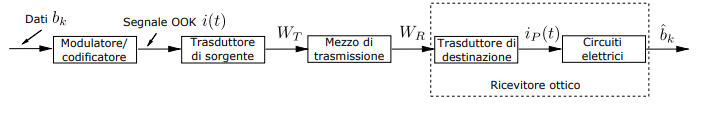
\includegraphics[width=\linewidth]{fbr.png}
    \caption{Schema generale}
\end{figure}

\noindent Gli elementi caratterizzanti sono:
\begin{itemize}
    \item Trasduttore di sorgente (Emettitore ottico)

        Ha il compito di generare un'onda elettromagnetica a frequenze ottiche partendo da una corrente d'ingresso, questo avviene in 2 modalità:
            \begin{enumerate}
                \item Emissione spontanea (LED)
                \item Emissione stimolata (LASER)\newline
            \end{enumerate}

        La potenza ottica trasmessa con corrente $i$ è:
        $$G\eta_i\eta_e\frac{i}{q}E_f$$
        \noindent In cui:
        \begin{itemize}
            \item $G$, guadagno d'amplificazione
            \item $\eta_i$, efficienza interna di generazione
            \item $\eta_e$, efficienza esterna di generazione
            \item $q$, carica dell'elettrone, $1.6*10^{-19}\ C$
            \item $E_f$, energia del fotone:
            $$h\frac{c}{\lambda}\text{ con } h=6.626*10^{-34}\ [J*s]$$
        \end{itemize}
        
    \item Mezzo di trasmissione
        \begin{itemize}
            \item Fibra ottica
            \item Mezzo wireless (Non approfondito qui)
        \end{itemize}
    \item Trasduttore di destinazione (Ricevitore ottico)
        \begin{itemize}
            \item Fotodiodo PIN
            \item Fotomoltiplicatore APD\newline
        \end{itemize}

        Dato un tempo di bit $T_b$ in cui l'energia totale ricevuta è $E_b$:
        $$N_{f/b}=\frac{E_b}{E_f}\ \text{ Num. medio fotoni per bit}$$
        \noindent A cui corrisponde:
        $$N_{f/s}=\frac{N_{f/b}}{T_b}\ \text{ Num. medio fotoni al secondo}$$
        \noindent Data $\eta$ probabilità che un fotone colpisca la giunzione, la corrente prodotta in uscita nei 2 casi sarà:
                $$i_{out}^{PIN}=\eta N_{f/s}q$$
                $$i_{out}^{APD}=G\eta N_{f/s}q$$\newline

        \noindent Affinché il ricevitore operi correttamente deve essere $N_{f/b}\geq \text{sensibilità ricevitore}$.\newline
        
\end{itemize}

\subsubsection{Propagazione}

La propagazione nella fibra ottica si basa sulla riflessione totale:

\begin{figure}[ht]
    \centering
    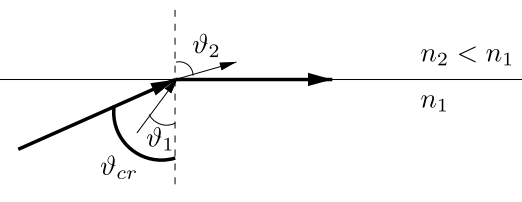
\includegraphics[width=0.7\linewidth]{rifl.png}
\end{figure}

\noindent Gli angoli e gli indici di rifrazione sono legati dalla legge di Snell:
$$\frac{\sin\vartheta_1}{\sin\vartheta_2}=\frac{n_2}{n_1}$$
\noindent L'angolo oltre il quale non c'è onda rifratta è dato da:
$$\arcsin\frac{n_2}{n_1}$$\newline

\noindent La fibra stessa è costruita in modo da innescare la riflessione totale:

\begin{figure}[ht]
    \centering
    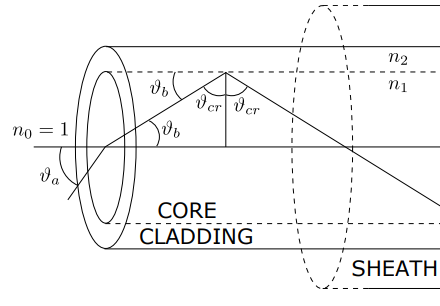
\includegraphics[width=0.6\linewidth]{fbr2.png}
\end{figure}

\noindent Per garantire il tutto deve essere $\vartheta_a<\arcsin(\sqrt{n_1^2-n_2^2})$.\newline

\df Il modo di propagazione è il percorso seguito dall'onda all'interno della fibra, il numero di modi si può approssimare con:
$$\frac{4}{\pi^2}\left(2\pi\frac{d_1}{2\lambda_0}\sqrt{n_1^2-n_2^2}\right)^2$$

\noindent In cui:
\begin{itemize}
    \item $d_1$, diametro del core
    \item $\lambda_0$, lunghezza d'onda utilizzata\newline
\end{itemize}

\noindent I fenomeni che limitano la distanza massima sono:
\begin{itemize}
    \item \textbf{Attenuazione}

        Legata a:
        \begin{itemize}
            \item Scattering di Rayleigh
            \item Ass. intrinseco
        \end{itemize}

        \newpage

        \noindent Ci sono 3 finestre di utilizzo della fibra:

        \begin{table}[ht]
            \centering
            \begin{tabular}{c|c|c|c|c}
                Finestra & $\lambda\ (\mu m)$ & $A_0\ (dB/Km)$ & $E_f\ (J)$ & Note\\
                \hline
                I & 0.85 & 2 & $2.34*10^{-19}$ & Usata per motivi storici\\
                \hline
                II & 1.33 & 0.3 & $1.49*10^{-19}$ & Min. dispersione\\
                \hline
                III & 1.55 & 0.2 & $1.28*10^{-19}$ & Min. attenuazione\\
            \end{tabular}
        \end{table}

        L'attenuazione introdotta in una fibra lunga $d_{Km}$ è calcolabile come:
        $$A_{dB}=A_0d_{Km}$$

    \item \textbf{Dispersione}

        Gli impulsi immessi si allargano temporalmente in base alla distanza, ci sono 2 cause:
        \begin{enumerate}
            \item \textbf{Modale}

                Causata dalla presenza di diversi modi, i fotoni seguono percorsi diversi ed arrivano in istanti diversi, si misura con il coefficiente:
                $$\delta_m\approx\frac{1}{\frac{c}{n_1}}\left(\frac{\sqrt{n_1^2-n_2^2}}{2n_1}\right)^2\ [s/Km]$$
                Che dopo $d_{Km}$ comporta un allargamento $\tau_m$ di $(d_{Km}\delta_m)$ metri.
            
            \item \textbf{Cromatica}

                Causata dalla presenza di diverse lunghezze d'onda nel segnale immesso, il coefficiente è:
                $$D=-\frac{\lambda d^2n}{cd\lambda^2}\ [ps/(nm*km)]$$
                Che dopo $d_{Km}$ comporta un allargamento $\tau_c$ di $(|D|d_{Km}\Delta\lambda)$ metri, $\Delta\lambda$ è la riga spettrale dell'emettitore.\newline
            
        \end{enumerate}
        
\end{itemize}

    \noindent Entrambe limitano il bitrate sostenibile ad una certa distanza:
    $$\displaystyle f_b<\frac{1}{\tau},\  f_b\leq\frac{W_T}{AShf}$$

\end{document}
